\section{Wohlstand}
\subsection{Die volkswirtschaftliche Diskussion}
\begin{itemize}
	\item Hoher Wohlstand
	\item Tiefe Arbeitslosigkeit
	\item Stabile Preise und Wechselkurse
	\item Nachhaltige Staatsfinanzierung
	\item Stabiles Finanzsystem
\end{itemize}
Dies sind die wirtschaftlichen Ziele eines Landes. Der Weg dazu führt entweder über Markt oder Staat.
\subsection{Makroökonomisches Grundmodell}
Das Makroökonomische gleichgewicht ist erreicht wenn die Kurven $AN$ und $AA_K$ sich bei der Kapazitätsgrenze schneiden. 
\begin{itemize}
	\item Preisniveau gemessen an definiertem Güterkorb
	\item Reales Bruttoinlandprodukt, inflationsbereinigte Wertschöpfung
\end{itemize}
	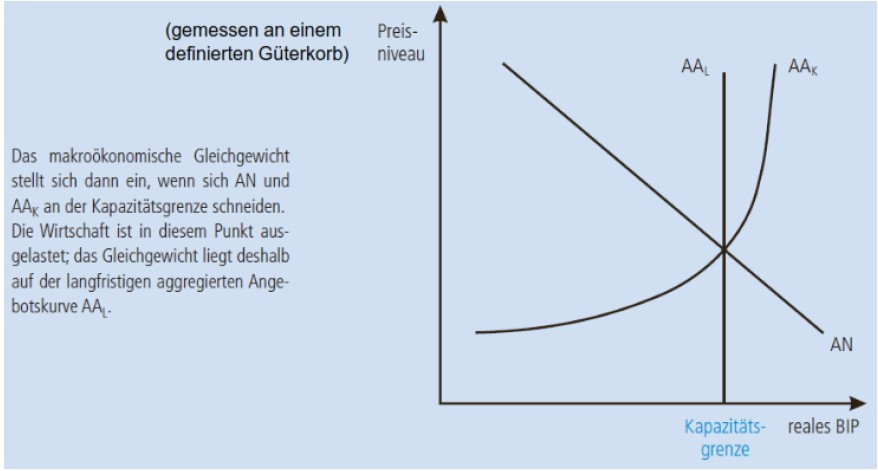
\includegraphics[width=0.85\linewidth]{images/makro.jpg}
	\subsubsection{aggregierte Nachfrage AN}
	Nachfrage nach Gütern (Waren und Dienstleistung) durch die vier volkswirtschaftlichen Akteure.
	\begin{itemize}
		\item Haushalt $\rightarrow$ Konsum
		\item Unternehmen $\rightarrow$ Investitionen
		\item Staat $\rightarrow$ Staatsausgaben
		\item Ausland $\rightarrow$ Nettoexporte = Exporte - Importe
	\end{itemize}
	\subsubsection{langfristig aggregiertes Angebot $AA_L$}
	Beziehung zwischen Produktionsfaktoren. Die Kapazitätsgrenze ist unabhängig vom Preisniveau.
	\begin{itemize}
		\item Arbeit
		\item Kapital
		\item Technologie
		\item Boden und Ressourcen
	\end{itemize}
	\subsubsection{kurzfristig aggregiertes Angebot $AA_K$}
	An der Kapazitätsgrenze sind die Produktionsfaktoren optimal, aber nicht maximal ausgelastet. Durch Überstunden und maximale Auslastung der Infrastruktur kann die $AA_K$-Kurve über der Kapazitätsgrenze liegen.
\subsection{Bruttoinlandprodukt (BIP)}
Das reale BIP (Nominales BIP inflationsbereinigt) der Schweiz beträgt 645 Mia. Franken. Um das BIP zu analysieren gibt es drei Ansätze
\begin{itemize}
	\item Produktionsansatz: Wertschöpfung der Wirschaftsakteure
	\item Einkommensansatz: Bezahlung der Produktionsfaktoren
	\item Verwendungsansatz: Wirtschaftssubjekte ihr Einkommen verwenden
\end{itemize}
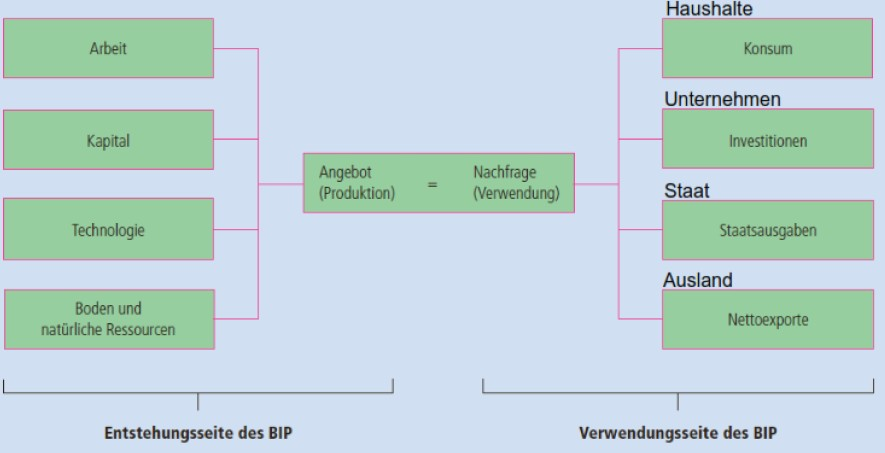
\includegraphics[width=0.9\linewidth]{images/bip.jpg}
\clearpage
\pagebreak